\chapter{System Engineering and Design}
\label{chap3}

\section{Introduction to System Architecture}
{
Figure \ref{fig:System} presents the complete system architecture, which consists of the following key components:

\begin{itemize}
\item ADXL335 accelerometer breakout board (analog sensor for vibration/time-domain data acquisition)
\item Arduino microcontroller (captures and preprocesses raw time-domain waveforms)
\item Raspberry Pi 4 microcomputer (performs frequency-domain transformation via FFT and manages database integration)
\end{itemize}

The system workflow enables end-to-end vibration monitoring, from analog signal acquisition to cloud-ready spectral analysis.

\begin{figure}[h]
\centering
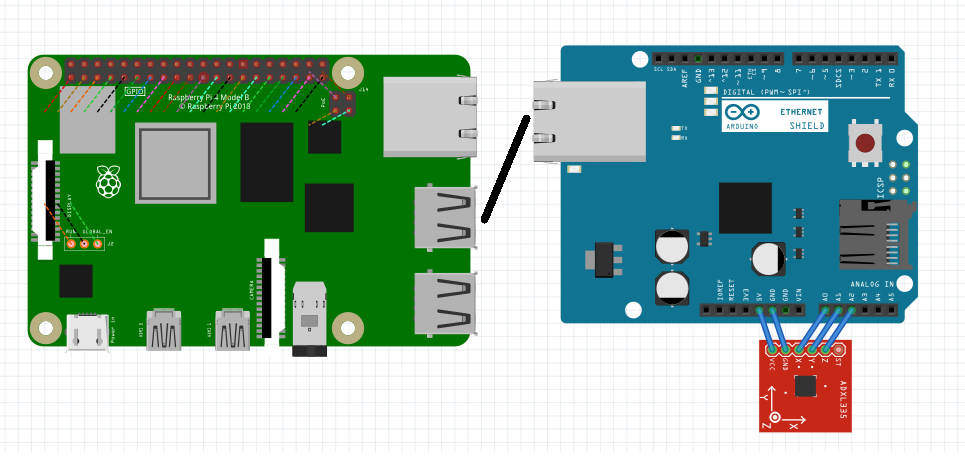
\includegraphics[width=\linewidth]{figures/System.png}
\caption{Full architecture overview}
\label{fig:System}
\end{figure}
}

\section{Algorithms}
\subsection{Arduino sketch}
{
Elaboration on (including the whole code):
\begin{itemize}
\item Description of sketch and cpp files
\item elaborate on how it shares data via UART
\item Analyse the possibility of translating Voltage into g or m/s2
\end{itemize}
}

\subsection{Raspberry Pi coding}
{
Elaboration on (including some parts of the code):
\begin{itemize}
\item Description of the whole program
\item how it posts data via HTTP
\item Data stored on database , and database setup
\end{itemize}
}

\subsection{Vercel coding}
{
Elaboration on (including some parts of the code):
\begin{itemize}
\item page file that prints data
\item how it is coupled with supabase
\end{itemize}
}
